\section{Example: Circuit Simulator}
\label{sec:ex}

%\lstset{
  captionpos=b,
  language=C++,
  basicstyle=\scriptsize,
  numbers=left,
  numberstyle=\tiny,
  columns=fullflexible,
  stepnumber=1,
  escapechar=\#,
  keepspaces=true,
  literate={<}{{$\langle$}}1 {>}{{$\rangle$}}1,
  morekeywords={region_relation,region,coloring,partition,spawn},
  deletekeywords=float,
}
\begin{lstlisting}[float={t},label={lst:code_ex},caption={Circuit Simulation Code Example}]
struct Node<rn>    { Node<rn>@rn next;    float charge, capacitance; }
struct Wire<rn,rn2,rw> { Wire<rn,rn2,rw>@rw next;
                                          Node<rn2>@rn in_node, out_node; float current, ... ; }
region_relation Circuit {
  region< Node<r_all_nodes> >                        r_all_nodes;
  region< Wire<r_all_nodes,r_all_nodes,r_all_wires> >       r_all_wires;
  Node<r_all_nodes>@r_all_nodes                   first_node;
  Wire<r_all_nodes,r_all_wires>@r_all_wires   first_wire;
}
region_relation CircuitPiece<rn, rw> {
  region< Node<rn_pvt+rn_shr> >                                 rn_pvt (#$\prec$# rn), rn_shr (#$\prec$# rn);
  region< Node<rn> >                                                   rn_ghost (#$\prec$# rn);
  region< Wire<rn_pvt+rn_shr+rn_ghost,rn,rw_pvt> >  rw_pvt (#$\prec$# rw);
  Node<rn_pvt+rn_shr>@(rn_pvt+rn_shr)                     first_node;
  Wire<rn_pvt+rn_shr+rn_ghost,rn,rw_pvt>@rw_pvt    first_wire;
};
void simulate_circuit(Circuit c) : RWE(c.r_all_nodes,c.r_all_wires)
{
  partition<c.r_all_wires> p_wires(wire_owner_map); // colored by piece they're in
  partition<c.r_all_nodes> p_nodes_pvs(node_sharing_map);
                                                                    // true = some neighbors in other pieces
  partition<p_nodes_pvs[false]> p_pvt_nodes(node_owner_map);
                                                                    // colored by piece they're in
  partition<p_nodes_pvs[true]> p_shr_nodes(node_owner_map);
                                                                    // colored by piece they're in
  partition<p_nodes_pvs[true]> p_ghost_nodes(node_nghbr_map);
                                                                    // colored by pieces they neighbor

  CircuitPiece<c.r_all_nodes,c.r_all_wires> pieces[MAX_PIECES];
  for(i = 0; i #$<$# MAX_PIECES; i++) 
    pieces[i] #$\gets$# { rn_pvt = p_pvt_nodes[i], rn_shr = p_shr_nodes[i],
                            rn_ghost = p_ghost_nodes[i], rw_pvt = p_wires[i] };

  while(!done) {
    for(i = 0; i #$<$# MAX_PIECES; i++) spawn calc_new_currents(pieces[i]);
    for(i = 0; i #$<$# MAX_PIECES; i++) spawn distribute_charge(pieces[i]);
    for(i = 0; i #$<$# MAX_PIECES; i++) spawn update_voltages(pieces[i]);
  }
}

// read info from nodes connected to each wire, update state of wire
void calc_new_currents(CircuitPiece<rn,rw> piece): RWE(piece.rw_pvt),
                                                                         ROE(piece.rn_pvt,piece.rn_ghost)

// current moving through wires redistributes charge between nodes
void distribute_charge(CircuitPiece<rn,rw> piece): ROE(piece.rw_pvt),
                                                                         RdA(piece.rn_pvt,piece.rn_ghost)

// total charge added to a node causes changes in voltage
void update_voltages(CircuitPiece<rn,rw> piece): RWE(piece.rn_pvt,piece.rn_shr)
\end{lstlisting}


In this section we give an informal overview of Legion through an example.
Listing~\ref{lst:code_ex} shows code for an electrical
circuit simulation, which illustrates the core features of the programming model.

The circuit simulation takes a collection of
of wires and nodes where wires meet.  
The simulation repeatedly updates
currents, distributes charges, and updates voltages for as many
time steps as the simulation demands.  We first
describe the partitioning of regions in Section~\ref{subsec:partitioning}
and then describe the data type declarations 
and the constraints they enforce on the simulation that enable
the runtime to efficiently execute the application
in Section~\ref{subsec:datatypes}.

\subsection{Regions and Partitions}
\label{subsec:partitioning}

Line 18 declares the main simulator function, which takes a {\tt
Circuit} to be simulated.  This function specifies the regions it 
accesses and the {\em privileges} and {\em coherence} it requires of those regions.
In this case, the {\tt RWE} annotation specifies that the function
accesses the regions {\tt c.r\_all\_nodes} and {\tt c.r\_all\_wires}
with read-write privileges and {\em exclusive} coherence (i.e., no other
function can access the regions concurrently).  The simulation 
reads and writes all nodes and wires, and it must be done
with exclusive access to ensure correct results.  Privileges specify what
the function can do with the regions; coherence specifies what other
functions can do with the regions concurrently.  Functions that
declare their accessed regions, privileges, and coherence are called {\em tasks}
and are the unit of parallel execution in Legion.

Lines 19-27 are responsible for partitioning the circuit into {\tt MAX\_PIECES}
pieces that can be worked on in parallel.  To partition a region, we
provide a {\em coloring}, which is a relation on the elements
of a region and a set of colors.  A {\em partition} is an object which given
a coloring and a region $r$ contains for each color $c$ a {\em subregion} of $r$
with all the elements of $r$ colored $c$.

The region of all nodes in the circuit is first partitioned into 
{\em private} and {\em shared} nodes (lines 20-21).  Private nodes
are touched by a single task in a phase, while shared nodes may
be referenced by multiple tasks in a phase.  The thick lines in figure \ref{sfig:part_fig:pvs}
show how the nodes in a small graph might be partitioned into three subsets.  Gray
nodes are shared and black nodes are private.  Note that
this partition is disjoint since each node has one color.
%Our current implementation uses small
%integers or booleans for the names of colors, but any enumerable set would be
%fine.  The coloring relation need not be total - it can leave out some elements entirely.  And although it is not required to be injective (it can map a single
%element to multiple colors), the fact that injective mappings will always
%result in disjoint subregions makes them strongly encouraged (when possible).
%Our example uses four colorings to create circuit partitions.

After partitioning into all the nodes that will be private and shared, we now
need to partition each of these subregions to generate {\tt MAX\_PIECES}-way
parallelism.  We first parition the private nodes into each of the disjoint
{\tt MAX\_PIECES} subregions (lines 23-24).  This partition can be seen in figure
\ref{sfig:part_fig:p_i}.  We similarly partition the shared subregion to
generate {\tt MAX\_PIECES} to correspond to the nodes that will be updated
by a each parallel computation.  This partitioning is also disjoint since
each node will only ever by updated by one parallel task and can be
seen in figure \ref{sfig:part_fig:s_i}.  Finally, we partition
the shared nodes again into the set of ghost nodes that we may want to make
multiple copies of since they will be read by multiple tasks.  Since
ghost nodes may be read by multiple parallel tasks, we may have to color
them multiple times and therefore the ghost partition is aliased
as can be seen in figure \ref{sfig:part_fig:g_i}.

Figure \ref{sfig:part_fig:tree} shows the final shape of the regions
and partitions.  The $*$ symbol indicates that a partition is 
disjoint.

%(These subsets are hopefully reasonably compact, but the correctness
%of the simulation is not dependent on that.)  
%Once the subsets are known, the \emph{node\_owner\_map} is created by assigning
%each node the color corresponding to its subset.  The 
%\emph{wire\_owner\_map} assigns each wire to the same subset as its ``in\_node''.
%The \emph{node\_nghbr\_map} maps a node to color(s) of all wires that 
%connect to it.  Finally, the \emph{node\_sharing\_map} is derived from the
%\emph{node\_nghbr\_map}, with a node colored ``true'' if any colors other than 
%its own were used, and ``false'' if the only wires that connect to a node are
%in the same piece.
%Figure~\ref{fig:part_fig} shows how the partitions are defined.

%Line 19 uses the \emph{wire\_owner\_map} to partition the wires region of the
%circuit into a subregion for each piece, but the partitioning of the nodes is
%more complicated due to the sharing that is necessary between the pieces.
%First, the \emph{node\_sharing\_map} is used to create two subregions: $p\_nodes\_pvs[false]$ contains all the nodes that are private to some piece (i.e. will
%never be needed for the computations in any other piece), while $p\_nodes\_pvs[true]$ contains nodes that will be accessed by multiple pieces' computations.
%Each of these subregions is then partitioned using the $node\_owner\_map$ to
%create the subregions owned by each computation.  These are the $p_i$ and $s_i$
%subregions, shown in Figures \ref{sfig:part_fig:p_i} and \ref{sfig:part_fig:s_i}.  Finally, the $g_i$ subregions (shown in Figure~\ref{sfig:part_fig:g_i}) are
%created using the $node\_nghbr\_map$ to 
%create subregions that include the ``ghost'' nodes needed to perform each
%piece's calculations.

With the partitioning operations completed, the various subregions are
recorded in an array of {\tt CircuitPiece} structures.  Lines 32-33 fill in multiple
fields of a {\tt CircuitPiece} at once.  The need for such a statement will be described in detail in 
section \ref{subsec:datatypes}.

%Because a region relationship can have
%fields with types that refer its own fields' values, it is often not possible
%to assign fields one at a time without violating the type checking rules.
%The simultaneous assignment operator asks the type checker only to make sure
%that the fields in the structure would have the right (self-referential) types
%after all the fields have been changed.

Lines 35-39 form the bulk of the actual simulation, performing three passes
over the circuit on each iteration.  For each pass, a for loop is used to 
spawn a task for each piece of the circuit.  There are no explicit requests for
parallel execution, nor is there explicit synchronization required between the
passes.  Both the fact that the pieces can be run in parallel for a single 
pass and the the required inter-task dependencies are determined automatically
by the runtime based on the region access annotations on the task declarations.
We will describe how this process occurs in more detail in section 
\ref{subsec:cirdependence}.

The declarations for the three subtasks are shown on lines 42-51.  The 
{\tt calc\_new\_currents} task declares that it will read and write the region containing wires
for that piece, and will need to read both the region containing nodes in its piece and any
node that is adjacent to the piece (i.e. the ghost node region).  
The {\tt distribute\_charge} subtask turns things around, reading the piece's 
region of wires and updating all the nodes that those wires connect to.  However,
rather than requesting the ability to read and write the nodes (which would
require serialization of these tasks for correctness), the task declares that
it will use reorderable reduction operations and that the coherence requirement
can be reduced to atomicity rather than exclusive access. The final task is 
{\tt update\_voltages}, in which each piece is able to update
voltage information on the nodes contained in regions that it owns (i.e. private and shared)
in that piece based on the reductions that happened in the previous task.  
  
%Since the wire subregions are known to be disjoint,
%the write sets of invocations of $calc\_new\_currents$ do not overlap, and can
%therefore be safely run in parallel.


%As long as the
%runtime can guarantee to apply the reductions from multiple subtasks safely, it
%can run the subtasks themselves in parallel.  Each invocation of 
%$distribute\_charge$ will be delayed until the corresponding invocation of 
%$calc\_new\_currents$ has completed due to the read-after-write dependency on
%the corresponding wire subregion.  However, despite the apparent 
%write-after-read anti-dependency on the ghost node regions, $distribute\_charge$
%tasks will generally not have to wait on the the completion of the other
%$calc\_new\_current$ tasks.  If there is sufficient memory available to make
%two copies of those nodes, the runtime can allow $distribute\_charge$ tasks to
%start calculating a new version of the nodes while older $calc\_new\_currents$
%tasks are still referring to the older version, all completely transparently to
%the application code.

%Again, the disjointness of the $p_i$ and $s_i$
%node subregions allows the runtime to safely run these tasks in parallel.  In
%this case, the runtime does wait for the completion of all the tasks in the 
%previous pass.  The read-after-write dependence on the $p_i$ is a guaranteed
%conflict, but there is also potential overlap between the $s_i$ subregions
%being reduced to in the previous pass and the $g_i$ subregions being accessed
%in this pass.  Although not every pair of $s_i$ and $g_j$ conflict, the
%runtime knows that they were created from two independent partitioning
%operations and guarantees correctness by conservatively assuming they might
%conflict.


\subsection{Data Types and Constraints}
\label{subsec:datatypes}
There are two primitive data types for the simulation: nodes
and wires.  {\tt Node}s are linked in a circular list.
To reflect that pointers from one {\tt Node} to the next stay
in the same region we use the {\tt Type@region} syntax (e.g.
the {\tt next} field on line 1).
The program relies on different lists being in different
regions, and the {\tt Node} definition is parameterized on a region
{\tt rn} to reflect this constraint.  
The {\tt next} field of a $\tt Node \langle rn \rangle$ has
type $\tt Node \langle rn \rangle \mbox{\tt @} rn$, which implies that
all nodes in the list are in region {\tt rn}.

{\tt Wire}s are similar, except that a wire refers to two nodes to
which it is electrically connected.  The two {\tt Node}s are in region {\tt rn},
but they may point to {\tt Node}s in a different region {\tt rn2}.  
This is a common pattern in Legion code, and
arises when a constraint needs to be placed on the objects directly
referenced, and a second (presumably weaker) constraint on objects
that are indirectly reached through the direct pointers.

In cases where we need to create compound data structures with types whose
region parameters are self-referential we declare a {\em region relationship}.
A region relationship is a structure with named fields, 
except that any region fields can be used in the type declarations
for other fields.  Lines 4-9 declare the region relationship {\tt Circuit}.
In {\tt Circuit} the region {\tt r\_all\_nodes} contains {\tt
Node}s that point only into region {\tt r\_all\_nodes}, guaranteeing that
all {\tt Node}s are in region {\tt r\_all\_nodes}.  (Note that regions are
declared with the single data type they can contain.)  Simiarly, the
type of the wire region's element not only guarantees that every wire
in the circuit is in the wire region, but also guarantees that every
node referred to by any wire is in the circuit's node region.

Since a region relationship can have
fields with types that refer its own fields' values, it is often not possible
to assign fields one at a time without violating the type checking rules.
The simultaneous assignment operator asks the type checker only to make sure
that the fields in the structure would have the right (self-referential) types
after all the fields have been changed.  Lines 32 and 33 illustrate a simultaneous
assignment to update a {\tt CircuitPiece} region relationship.

The last type definition is for the pieces into which the circuit is partitioned.
The original node and wire regions are specified as parameters, and the
four kinds of subregions that are created are made fields of the
{\tt CircuitPiece} (lines 10-17).  This declaration also illustrates {\em subregion constraints}
placed on the three region fields stating the region fields must be subregions of the 
node and wire regions provided as parameters (line 16).  Since the simulation code will need to be able to
iterate over the nodes owned by a {\tt CircuitPiece}, the parameterization of the {\tt rn\_pvt} (private nodes),
{\tt rn\_shr} (shared nodes), and {\tt first\_node} fields constrains the linked list of
nodes to reside entirely in those two regions.  The linked list of wires is
similarly constrained, and the wire's node pointers are constrained to fall
into one of the three subregions defined in the {\tt CircuitPiece}.  Finally,
the use of {\tt rn} for {\tt rn\_ghost}'s parameter and the second parameter
in the wire type places no constraints on which nodes a ghost node might point
to.


%\def\partitiontree{
%\draw[step=0.5,gray,very thin] (0,0) grid (8,5);

\node(top) at (3.5,4.5) { $all{\_}nodes$ };

\node(pvsf) at (2,2.5) { $pvs[false]$ };
\node(pvst) at (5,2.5) { $pvs[true]$ };

\node(p0) at (0.7,0.5) { $p_0$ };
\node(p1) at (1.2,0.5) { $p_1$ };
\node(pd) at (1.6,0.5) { $\ldots$ };
\node(pn) at (2.3,0.5) { $p_{n-1}$ };

\node(s0) at (3.2,0.5) { $s_0$ };
\node(s1) at (3.7,0.5) { $s_1$ };
\node(sd) at (4.1,0.5) { $\ldots$ };
\node(sn) at (4.8,0.5) { $s_{n-1}$ };

\node(g0) at (5.7,0.5) { $g_0$ };
\node(g1) at (6.2,0.5) { $g_1$ };
\node(gd) at (6.6,0.5) { $\ldots$ };
\node(gn) at (7.3,0.5) { $g_{n-1}$ };

\draw[xshift=3.5cm,yshift=3.5cm] (-1,0) -- (1,0)
  node(ptf)[pos=0.25,inner sep=0] {} edge (pvsf.north)
  node[pos=0.5,anchor=south east] {$*$}
  node(ptp)[pos=0.5,inner sep=0] {} edge (top.south)
  node(ptt)[pos=0.75,inner sep=0] {} edge (pvst.north)
  ;

\draw[xshift=1.5cm,yshift=1.5cm] (-1,0) -- (1,0)
  node(pp0)[pos=0.2,inner sep=0] {} edge (p0.north)
  node(pp1)[pos=0.4,inner sep=0] {} edge (p1.north)
  node[pos=0.5,anchor=south east] {$*$}
  node(ppp)[pos=0.5,inner sep=0] {} edge (pvsf.250)
  node(ppn)[pos=0.8,inner sep=0] {} edge (pn.north)
  ;

\draw[xshift=4cm,yshift=1.5cm] (-1,0) -- (1,0)
  node(ps0)[pos=0.2,inner sep=0] {} edge (s0.north)
  node(ps1)[pos=0.4,inner sep=0] {} edge (s1.north)
  node[pos=0.5,anchor=south east] {$*$}
  node(psp)[pos=0.5,inner sep=0] {} edge (pvst.230)
  node(psn)[pos=0.8,inner sep=0] {} edge (sn.north)
  ;

\draw[xshift=6.5cm,yshift=1.5cm] (-1,0) -- (1,0)
  node(pg0)[pos=0.2,inner sep=0] {} edge (g0.north)
  node(pg1)[pos=0.4,inner sep=0] {} edge (g1.north)
  node[pos=0.5,anchor=south east] {}
  node(pgp)[pos=0.5,inner sep=0] {} edge (pvst.310)
  node(pgn)[pos=0.8,inner sep=0] {} edge (gn.north)
  ;
}

\def\partitiongraph{
%\draw[step=0.5,gray,very thin] (0,0) grid (8,5);

\node[cn,s0] (n1) at (0.77,1.27) {};
\node[cn,p0] (n2) at (1.6165,3.3865) {};
\node[cn,s0] (n3) at (2.463,2.54) {};
\node[cn,p0] (n4) at (0.8755,2.54) {};
\node[cn,p2] (n5) at (2.463,0.529) {};
\node[cn,s2] (n6) at (3.945,1.799) {};
\node[cn,s0] (n7) at (3.6275,2.963) {};
\node[cn,p2] (n8) at (4.7915,0.529) {};
\node[cn,s1] (n9) at (5.638,1.5875) {};
\node[cn,s1] (n10) at (6.6965,1.164) {};
\node[cn,s1] (n11) at (5.215,2.6455) {};
\node[cn,p1] (n12) at (6.379,2.7515) {};
\node[cn,p1] (n13) at (5.3205,3.598) {};
\node[cn,s1,g0] (n14) at (4.1565,4.1275) {};
\node[cn,s0] (n15) at (2.8865,3.81) {};
\node[cn,p0] (n16) at (0.77,4.1275) {};
\node[cn,s2,g0] (n17) at (1.405,0.423) {};
\node[cn,p1] (n18) at (6.379,4.0215) {};
\node[cn,s2,g0] (n19) at (2.7805,1.4815) {};
\node[cn,s0] (n20) at (1.7225,1.799) {};
\node[cn,p2] (n21) at (3.733,0.7405) {};
\node[cn,s2] (n22) at (5.85,0.635) {};

\draw (n16) to (n2);
\draw (n16) to (n4);
\draw (n5) to (n21);
\draw (n21) to (n8);
\draw (n12) to (n13) to (n18) to (n12);


\draw[p2s] (n1) to (n4) to (n20);
\draw[p2s] (n4) to (n3) to (n15) to (n2);
\draw[p2s] (n15) to (n7);

\draw[p2s] (n14) to (n13) to (n11) to (n9) to (n12) to (n10);

\draw[p2s] (n17) to (n19) to (n5);
\draw[p2s] (n19) to (n6) to (n8) to (n22);

\draw[s2s] (n1) to (n17);
\draw[s2s] (n20) to (n19) to (n3);
\draw[s2s] (n15) to (n14) to (n7);
\draw[s2s] (n11) to (n6) to (n9) to (n22) to (n10);

\draw[thick] (0.5,0.5) to (4,2.5);
\draw[thick] (3.75,4.5) to (4,2.5);
\draw[thick] (6.5,0.5) to (4,2.5);

\draw[dashed] (0.5,1.5) .. controls (1,2) and (1.5,2.5) .. (1.9,3.1) .. controls (2,4) .. (1.75,4.5);
\draw[dashed] (5.25,4.5) .. controls (4.75,3.5) .. (5.25,3.25) .. controls (6,3) .. (6,2.5) .. controls (6,2.25) .. (7,2.5);
\draw[dashed] (2,0.25) .. controls (2.25,1) .. (3.5,1.1) .. controls (5,1.25) .. (5.5,0.25);
}

\begin{figure}[t]
  \centering
\subfigure[partitioning tree]{
\label{sfig:part_fig:tree}
\begin{tikzpicture}[scale=0.8]
\partitiontree
\end{tikzpicture}
}

  \subfigure[$pvs$]{
\label{sfig:part_fig:pvs}
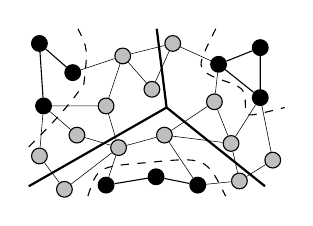
\begin{tikzpicture}
  [scale=0.5, cn/.style={circle,draw,inner sep=0,minimum size=2mm},
   p0/.style={fill},
   p1/.style={fill},
   p2/.style={fill},
   s0/.style={fill=lightgray},
   s1/.style={fill=lightgray},
   s2/.style={fill=lightgray},
   g0/.style={},
   p2p/.style={very thin},
   p2s/.style={very thin},
   s2s/.style={very thin}]
\partitiongraph
\end{tikzpicture}
}
  \subfigure[$p_i$]{
\label{sfig:part_fig:p_i}
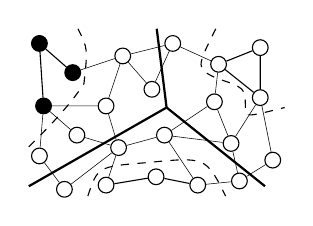
\begin{tikzpicture}
  [scale=0.5, cn/.style={circle,draw,inner sep=0,minimum size=2mm},
   p0/.style={fill},
   p1/.style={},
   p2/.style={},
   s0/.style={},
   s1/.style={},
   s2/.style={},
   g0/.style={},
   p2p/.style={very thin},
   p2s/.style={very thin},
   s2s/.style={very thin}]
\partitiongraph
\end{tikzpicture}
}
  \subfigure[$s_i$]{
\label{sfig:part_fig:s_i}
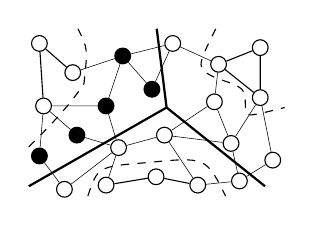
\begin{tikzpicture}
  [scale=0.5, cn/.style={circle,draw,inner sep=0,minimum size=2mm},
   p0/.style={},
   p1/.style={},
   p2/.style={},
   s0/.style={fill},
   s1/.style={},
   s2/.style={},
   g0/.style={},
   p2p/.style={very thin},
   p2s/.style={very thin},
   s2s/.style={very thin}]
\partitiongraph
\end{tikzpicture}
}
  \subfigure[$g_i$]{
\label{sfig:part_fig:g_i}
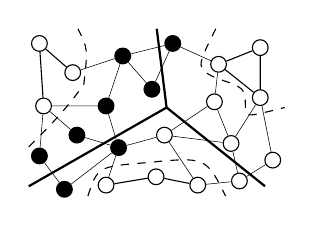
\begin{tikzpicture}
  [scale=0.5, cn/.style={circle,draw,inner sep=0,minimum size=2mm},
   p0/.style={},
   p1/.style={},
   p2/.style={},
   s0/.style={fill},
   s1/.style={},
   s2/.style={},
   g0/.style={fill},
   p2p/.style={very thin},
   p2s/.style={very thin},
   s2s/.style={very thin}]
\partitiongraph
\end{tikzpicture}
}
  \label{fig:part_fig}
  \caption{Partitions of $r{\_}all{\_}nodes$}
%  \caption[My caption
\end{figure}


%\lstset{
  captionpos=b,
  language=C++,
  basicstyle=\scriptsize,
  numbers=left,
  numberstyle=\tiny,
  columns=fullflexible,
  stepnumber=1,
  escapechar=\#,
  keepspaces=true,
  literate={<}{{$\langle$}}1 {>}{{$\rangle$}}1,
  morekeywords={region_relation,region,coloring,partition,spawn},
  deletekeywords=float,
}
\begin{lstlisting}[float={t},label={lst:code_ex},caption={Circuit Simulation Code Example}]
struct Node<rn>    { Node<rn>@rn next;    float charge, capacitance; }
struct Wire<rn,rn2,rw> { Wire<rn,rn2,rw>@rw next;
                                          Node<rn2>@rn in_node, out_node; float current, ... ; }
region_relation Circuit {
  region< Node<r_all_nodes> >                        r_all_nodes;
  region< Wire<r_all_nodes,r_all_nodes,r_all_wires> >       r_all_wires;
  Node<r_all_nodes>@r_all_nodes                   first_node;
  Wire<r_all_nodes,r_all_wires>@r_all_wires   first_wire;
}
region_relation CircuitPiece<rn, rw> {
  region< Node<rn_pvt+rn_shr> >                                 rn_pvt (#$\prec$# rn), rn_shr (#$\prec$# rn);
  region< Node<rn> >                                                   rn_ghost (#$\prec$# rn);
  region< Wire<rn_pvt+rn_shr+rn_ghost,rn,rw_pvt> >  rw_pvt (#$\prec$# rw);
  Node<rn_pvt+rn_shr>@(rn_pvt+rn_shr)                     first_node;
  Wire<rn_pvt+rn_shr+rn_ghost,rn,rw_pvt>@rw_pvt    first_wire;
};
void simulate_circuit(Circuit c) : RWE(c.r_all_nodes,c.r_all_wires)
{
  partition<c.r_all_wires> p_wires(wire_owner_map); // colored by piece they're in
  partition<c.r_all_nodes> p_nodes_pvs(node_sharing_map);
                                                                    // true = some neighbors in other pieces
  partition<p_nodes_pvs[false]> p_pvt_nodes(node_owner_map);
                                                                    // colored by piece they're in
  partition<p_nodes_pvs[true]> p_shr_nodes(node_owner_map);
                                                                    // colored by piece they're in
  partition<p_nodes_pvs[true]> p_ghost_nodes(node_nghbr_map);
                                                                    // colored by pieces they neighbor

  CircuitPiece<c.r_all_nodes,c.r_all_wires> pieces[MAX_PIECES];
  for(i = 0; i #$<$# MAX_PIECES; i++) 
    pieces[i] #$\gets$# { rn_pvt = p_pvt_nodes[i], rn_shr = p_shr_nodes[i],
                            rn_ghost = p_ghost_nodes[i], rw_pvt = p_wires[i] };

  while(!done) {
    for(i = 0; i #$<$# MAX_PIECES; i++) spawn calc_new_currents(pieces[i]);
    for(i = 0; i #$<$# MAX_PIECES; i++) spawn distribute_charge(pieces[i]);
    for(i = 0; i #$<$# MAX_PIECES; i++) spawn update_voltages(pieces[i]);
  }
}

// read info from nodes connected to each wire, update state of wire
void calc_new_currents(CircuitPiece<rn,rw> piece): RWE(piece.rw_pvt),
                                                                         ROE(piece.rn_pvt,piece.rn_ghost)

// current moving through wires redistributes charge between nodes
void distribute_charge(CircuitPiece<rn,rw> piece): ROE(piece.rw_pvt),
                                                                         RdA(piece.rn_pvt,piece.rn_ghost)

// total charge added to a node causes changes in voltage
void update_voltages(CircuitPiece<rn,rw> piece): RWE(piece.rn_pvt,piece.rn_shr)
\end{lstlisting}

%\def\partitiontree{
%\draw[step=0.5,gray,very thin] (0,0) grid (8,5);

\node(top) at (3.5,4.5) { $all{\_}nodes$ };

\node(pvsf) at (2,2.5) { $pvs[false]$ };
\node(pvst) at (5,2.5) { $pvs[true]$ };

\node(p0) at (0.7,0.5) { $p_0$ };
\node(p1) at (1.2,0.5) { $p_1$ };
\node(pd) at (1.6,0.5) { $\ldots$ };
\node(pn) at (2.3,0.5) { $p_{n-1}$ };

\node(s0) at (3.2,0.5) { $s_0$ };
\node(s1) at (3.7,0.5) { $s_1$ };
\node(sd) at (4.1,0.5) { $\ldots$ };
\node(sn) at (4.8,0.5) { $s_{n-1}$ };

\node(g0) at (5.7,0.5) { $g_0$ };
\node(g1) at (6.2,0.5) { $g_1$ };
\node(gd) at (6.6,0.5) { $\ldots$ };
\node(gn) at (7.3,0.5) { $g_{n-1}$ };

\draw[xshift=3.5cm,yshift=3.5cm] (-1,0) -- (1,0)
  node(ptf)[pos=0.25,inner sep=0] {} edge (pvsf.north)
  node[pos=0.5,anchor=south east] {$*$}
  node(ptp)[pos=0.5,inner sep=0] {} edge (top.south)
  node(ptt)[pos=0.75,inner sep=0] {} edge (pvst.north)
  ;

\draw[xshift=1.5cm,yshift=1.5cm] (-1,0) -- (1,0)
  node(pp0)[pos=0.2,inner sep=0] {} edge (p0.north)
  node(pp1)[pos=0.4,inner sep=0] {} edge (p1.north)
  node[pos=0.5,anchor=south east] {$*$}
  node(ppp)[pos=0.5,inner sep=0] {} edge (pvsf.250)
  node(ppn)[pos=0.8,inner sep=0] {} edge (pn.north)
  ;

\draw[xshift=4cm,yshift=1.5cm] (-1,0) -- (1,0)
  node(ps0)[pos=0.2,inner sep=0] {} edge (s0.north)
  node(ps1)[pos=0.4,inner sep=0] {} edge (s1.north)
  node[pos=0.5,anchor=south east] {$*$}
  node(psp)[pos=0.5,inner sep=0] {} edge (pvst.230)
  node(psn)[pos=0.8,inner sep=0] {} edge (sn.north)
  ;

\draw[xshift=6.5cm,yshift=1.5cm] (-1,0) -- (1,0)
  node(pg0)[pos=0.2,inner sep=0] {} edge (g0.north)
  node(pg1)[pos=0.4,inner sep=0] {} edge (g1.north)
  node[pos=0.5,anchor=south east] {}
  node(pgp)[pos=0.5,inner sep=0] {} edge (pvst.310)
  node(pgn)[pos=0.8,inner sep=0] {} edge (gn.north)
  ;
}

\def\partitiongraph{
%\draw[step=0.5,gray,very thin] (0,0) grid (8,5);

\node[cn,s0] (n1) at (0.77,1.27) {};
\node[cn,p0] (n2) at (1.6165,3.3865) {};
\node[cn,s0] (n3) at (2.463,2.54) {};
\node[cn,p0] (n4) at (0.8755,2.54) {};
\node[cn,p2] (n5) at (2.463,0.529) {};
\node[cn,s2] (n6) at (3.945,1.799) {};
\node[cn,s0] (n7) at (3.6275,2.963) {};
\node[cn,p2] (n8) at (4.7915,0.529) {};
\node[cn,s1] (n9) at (5.638,1.5875) {};
\node[cn,s1] (n10) at (6.6965,1.164) {};
\node[cn,s1] (n11) at (5.215,2.6455) {};
\node[cn,p1] (n12) at (6.379,2.7515) {};
\node[cn,p1] (n13) at (5.3205,3.598) {};
\node[cn,s1,g0] (n14) at (4.1565,4.1275) {};
\node[cn,s0] (n15) at (2.8865,3.81) {};
\node[cn,p0] (n16) at (0.77,4.1275) {};
\node[cn,s2,g0] (n17) at (1.405,0.423) {};
\node[cn,p1] (n18) at (6.379,4.0215) {};
\node[cn,s2,g0] (n19) at (2.7805,1.4815) {};
\node[cn,s0] (n20) at (1.7225,1.799) {};
\node[cn,p2] (n21) at (3.733,0.7405) {};
\node[cn,s2] (n22) at (5.85,0.635) {};

\draw (n16) to (n2);
\draw (n16) to (n4);
\draw (n5) to (n21);
\draw (n21) to (n8);
\draw (n12) to (n13) to (n18) to (n12);


\draw[p2s] (n1) to (n4) to (n20);
\draw[p2s] (n4) to (n3) to (n15) to (n2);
\draw[p2s] (n15) to (n7);

\draw[p2s] (n14) to (n13) to (n11) to (n9) to (n12) to (n10);

\draw[p2s] (n17) to (n19) to (n5);
\draw[p2s] (n19) to (n6) to (n8) to (n22);

\draw[s2s] (n1) to (n17);
\draw[s2s] (n20) to (n19) to (n3);
\draw[s2s] (n15) to (n14) to (n7);
\draw[s2s] (n11) to (n6) to (n9) to (n22) to (n10);

\draw[thick] (0.5,0.5) to (4,2.5);
\draw[thick] (3.75,4.5) to (4,2.5);
\draw[thick] (6.5,0.5) to (4,2.5);

\draw[dashed] (0.5,1.5) .. controls (1,2) and (1.5,2.5) .. (1.9,3.1) .. controls (2,4) .. (1.75,4.5);
\draw[dashed] (5.25,4.5) .. controls (4.75,3.5) .. (5.25,3.25) .. controls (6,3) .. (6,2.5) .. controls (6,2.25) .. (7,2.5);
\draw[dashed] (2,0.25) .. controls (2.25,1) .. (3.5,1.1) .. controls (5,1.25) .. (5.5,0.25);
}

\begin{figure}[t]
  \centering
\subfigure[partitioning tree]{
\label{sfig:part_fig:tree}
\begin{tikzpicture}[scale=0.8]
\partitiontree
\end{tikzpicture}
}

  \subfigure[$pvs$]{
\label{sfig:part_fig:pvs}
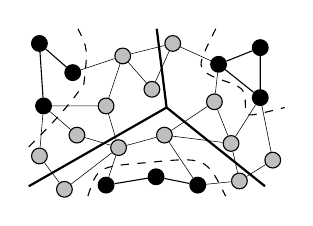
\begin{tikzpicture}
  [scale=0.5, cn/.style={circle,draw,inner sep=0,minimum size=2mm},
   p0/.style={fill},
   p1/.style={fill},
   p2/.style={fill},
   s0/.style={fill=lightgray},
   s1/.style={fill=lightgray},
   s2/.style={fill=lightgray},
   g0/.style={},
   p2p/.style={very thin},
   p2s/.style={very thin},
   s2s/.style={very thin}]
\partitiongraph
\end{tikzpicture}
}
  \subfigure[$p_i$]{
\label{sfig:part_fig:p_i}
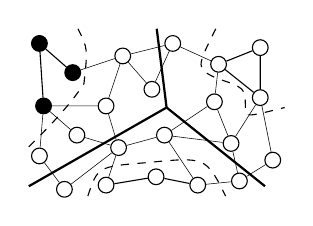
\begin{tikzpicture}
  [scale=0.5, cn/.style={circle,draw,inner sep=0,minimum size=2mm},
   p0/.style={fill},
   p1/.style={},
   p2/.style={},
   s0/.style={},
   s1/.style={},
   s2/.style={},
   g0/.style={},
   p2p/.style={very thin},
   p2s/.style={very thin},
   s2s/.style={very thin}]
\partitiongraph
\end{tikzpicture}
}
  \subfigure[$s_i$]{
\label{sfig:part_fig:s_i}
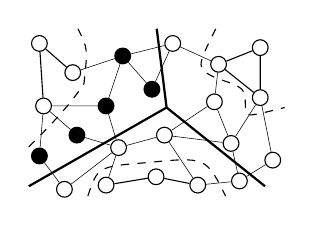
\begin{tikzpicture}
  [scale=0.5, cn/.style={circle,draw,inner sep=0,minimum size=2mm},
   p0/.style={},
   p1/.style={},
   p2/.style={},
   s0/.style={fill},
   s1/.style={},
   s2/.style={},
   g0/.style={},
   p2p/.style={very thin},
   p2s/.style={very thin},
   s2s/.style={very thin}]
\partitiongraph
\end{tikzpicture}
}
  \subfigure[$g_i$]{
\label{sfig:part_fig:g_i}
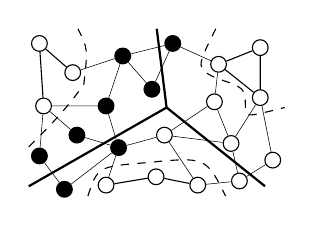
\begin{tikzpicture}
  [scale=0.5, cn/.style={circle,draw,inner sep=0,minimum size=2mm},
   p0/.style={},
   p1/.style={},
   p2/.style={},
   s0/.style={fill},
   s1/.style={},
   s2/.style={},
   g0/.style={fill},
   p2p/.style={very thin},
   p2s/.style={very thin},
   s2s/.style={very thin}]
\partitiongraph
\end{tikzpicture}
}
  \label{fig:part_fig}
  \caption{Partitions of $r{\_}all{\_}nodes$}
%  \caption[My caption
\end{figure}

